\begin{frame}{Example: Step 1}
	$M = (r, ph, r)$, $UNEQUAL(0, 2)$
	
	\begin{itemize}
		\item Optimal route found with PNE: $(r_1, ph_1, r_1)$
	\end{itemize}
	
	\begin{figure}[h]
		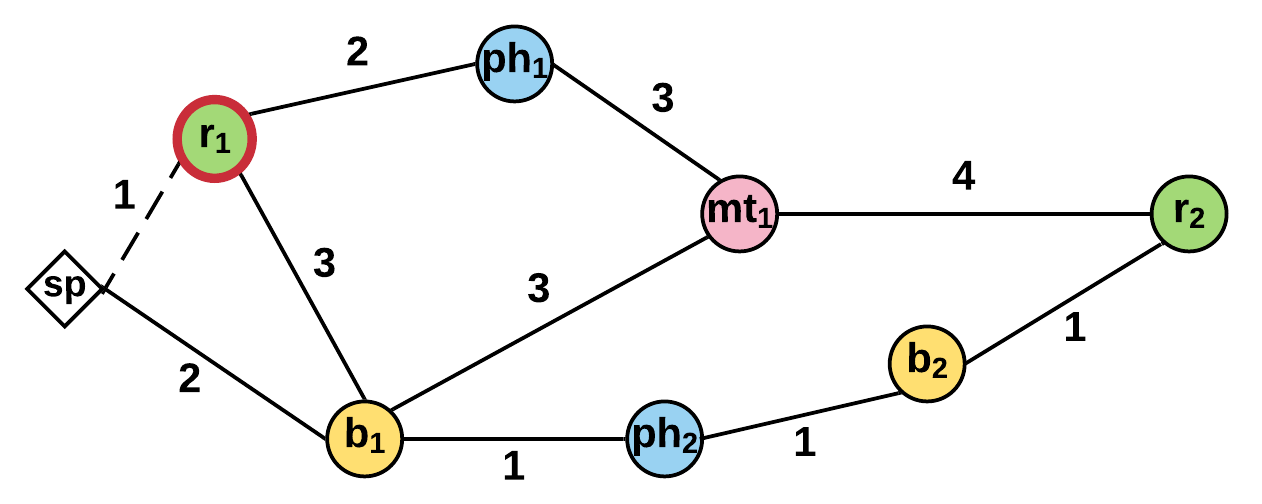
\includegraphics[scale=0.8]{Example_NEO_1.png}
	\end{figure}
	
	\begin{table}[h]
		\centering
		\begin{tabular}{ |l|p{10cm}| } 
			\hline
			Step & Heap contents (PSR $R : length(R)$) \\
			\hline
			\textcolor{red}{1} & \textcolor{red}{$(r_1 : 1)$} \\ 
			\hline
		\end{tabular}
	\end{table}

\end{frame}

\begin{frame}{Example: Step 2}
	$M = (r, ph, r)$, $UNEQUAL(0, 2)$
	
	\begin{figure}[h]
		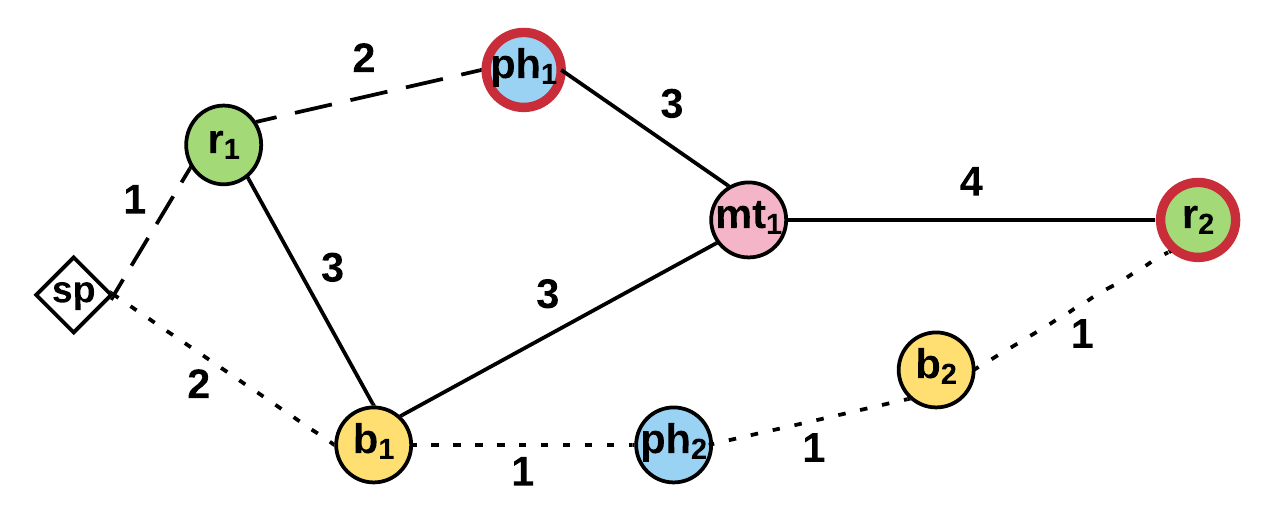
\includegraphics[scale=0.8]{Example_NEO_2.png}
	\end{figure}
	
	\begin{table}[h]
		\centering
		\begin{tabular}{ |l|p{10cm}| } 
			\hline
			Step & Heap contents (PSR $R : length(R)$) \\
			\hline
			1 & $(r_1 : 1)$ \\ 
			\hline
			\textcolor{red}{2} & \textcolor{red}{$(r_1, ph_1 : 3)$}, \textcolor{red}{$(r_2 : 5)$} \\ 
			\hline
		\end{tabular}
	\end{table}

\end{frame}

\begin{frame}{Example: Step 3}
	$M = (r, ph, r)$, $UNEQUAL(0, 2)$
	
	\begin{figure}[h]
		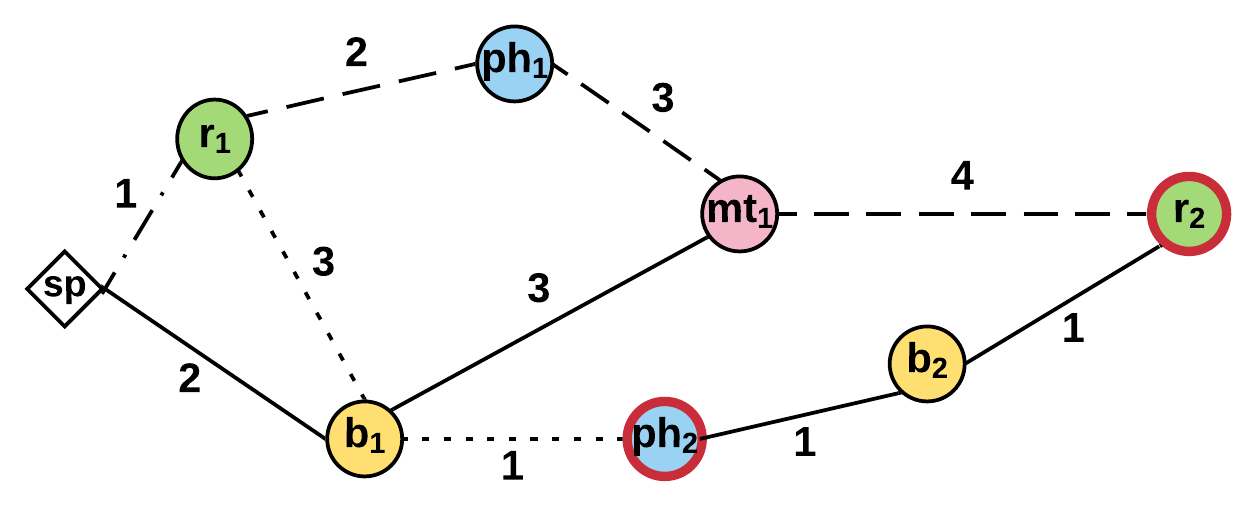
\includegraphics[scale=0.8]{Example_NEO_3.png}
	\end{figure}
	
	\begin{table}[h]
		\centering
		\begin{tabular}{ |l|p{10cm}| } 
			\hline
			Step & Heap contents (PSR $R : length(R)$) \\
			\hline
			2 & $(r_1, ph_1 : 3), (r_2 : 5)$ \\ 
			\hline
			\textcolor{red}{3} & $(r_2 : 5), $ \textcolor{red}{$(r_1, ph_2 : 5)$}, \textcolor{red}{$(r_1, ph_1, r_2 : 10)$} \\
			\hline 
		\end{tabular}
	\end{table}

\end{frame}

\begin{frame}{Example: Step 5}
	$M = (r, ph, r)$, $UNEQUAL(0, 2)$
	
	\begin{figure}[h]
		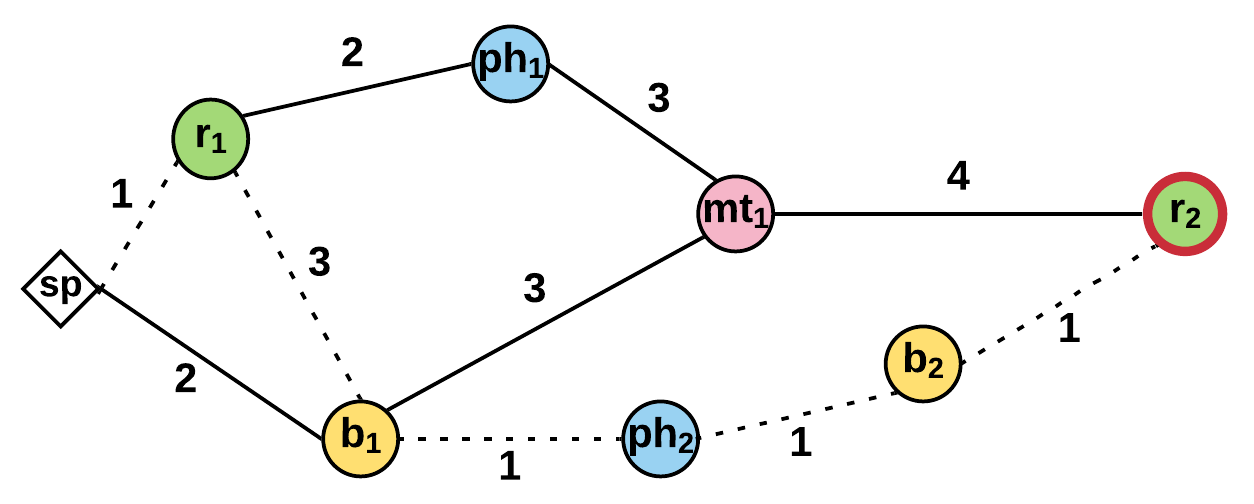
\includegraphics[scale=0.8]{Example_NEO_5.png}
	\end{figure}
	
	\begin{table}[h]
		\centering
		\begin{tabular}{ |l|p{10cm}| } 
			\hline
			Step & Heap contents (PSR $R : length(R)$) \\
			\hline
			4 & $(r_1, ph_2 : 5), (r_2, ph_2 : 7), (r_1, ph_1, r_2 : 10)$ \\ 
			\hline
			\textcolor{red}{5} & \textcolor{red}{$(r_1, ph_2, r_2 : 7)$}, $(r_2, ph_2 : 7),$ \st{$(r_1, ph_1, r_2 : 10)$} \\ 
			\hline
		\end{tabular}
	\end{table}

\end{frame}

%\begin{frame}{Example}
%	\begin{table}[]
%		\centering
%		\begin{tabular}{ |l|l| } 
%			\hline
%			Step & Heap contents (PSR $R : length(R)$) \\
%			\hline
%			1 & $(r_1 : 1)$ \\ 
%			\hline
%			2 & $(r_1, ph_1 : 3), (r_2 : 5)$ \\ 
%			\hline
%			3 & $(r_2 : 5), (r_1, ph_2 : 5), (r_1, ph_1, r_2 : 10)$ \\ 
%			\hline
%			4 & $(r_1, ph_2 : 5), (r_2, ph_2 : 7), (r_1, ph_1, r_2 : 10)$ \\ 
%			\hline
%			5 & $(r_1, ph_2, r_2 : 7), (r_2, ph_2 : 7), (r_1, ph_1, r_2 : 10)$ \\ 
%			\hline
%		\end{tabular}
%	\end{table}
%\end{frame}